\chapter{Results}
%Plan
We begin this chapter showcasing a series of canonical results from the {\sc meqsilhouette} simulator. 
%awaiting
Following this we attempt awith more sophisticated results of calibrator and imaging tests of a variable source within the context of a variable troposphere, with possibly some ISM thrown in.
%link to design objectives
Apparent in these results is the realisation of the design objectives laid out \ref{sec:

\section{Canonical simulations}\label{sec:can_sim}




\subsection{ISM}


% Link to diagram in ISM:theory about redoing the Ortiz-leon plot. This is a verification of a large section of the simulator
The reproduction of the \citet{Ortiz_2016} result in Fig.~\ref{fig:substructure2} verifies a large section of the simulation modules, including the interferometric simulation and the ISM simulation module. This also shows the flexibility of the software.




% ISM sequence
To demonstrate the implementation and provide an example of intraday ISM variability, we present the results of a simulated observation of 10 minutes duration at 14:00 UTC on four consecutive days in Fig.~\ref{ISM_sequence}. To compare to published observations, we use the three-station EHT array consisting of the Submillimeter Telescope (SMT) in Arizona, the Combined Array for Research in Millimeter-wave Astronomy (CARMA) in California and the James Clerk Maxwell Telescope (JCMT) on Mauna Kea, Hawaii. The distance to the screen is taken as $D_{\rm os}=5.8 \pm 0.3$~kpc  \citep{Bower_2014}. The relative transverse velocity between the observer and scattering screen is set to $50~\rm{km\,s}^{-1}$ to be consistent with \citet{2016arXiv160106571O}. The source is a circular Gaussian with a $\rm{FHWM}=40$~$\mu$-arcsec, approximately the angular distance that a scattering screen would travel over $\sim 4$~days. The source size has been chosen such that it is consistent with the latest estimate of the size of Sgr~A$^\star$ at $230$~GHz \citep{Fish_2011}.  Closure quantities are model dependent and calculated as specified in \citet{Rogers_1995}, where the thermal noise was added based on the system equivalent flux density (SEFD) table in \citep{Lu_2014}. 


\begin{figure*}
\begin{center}
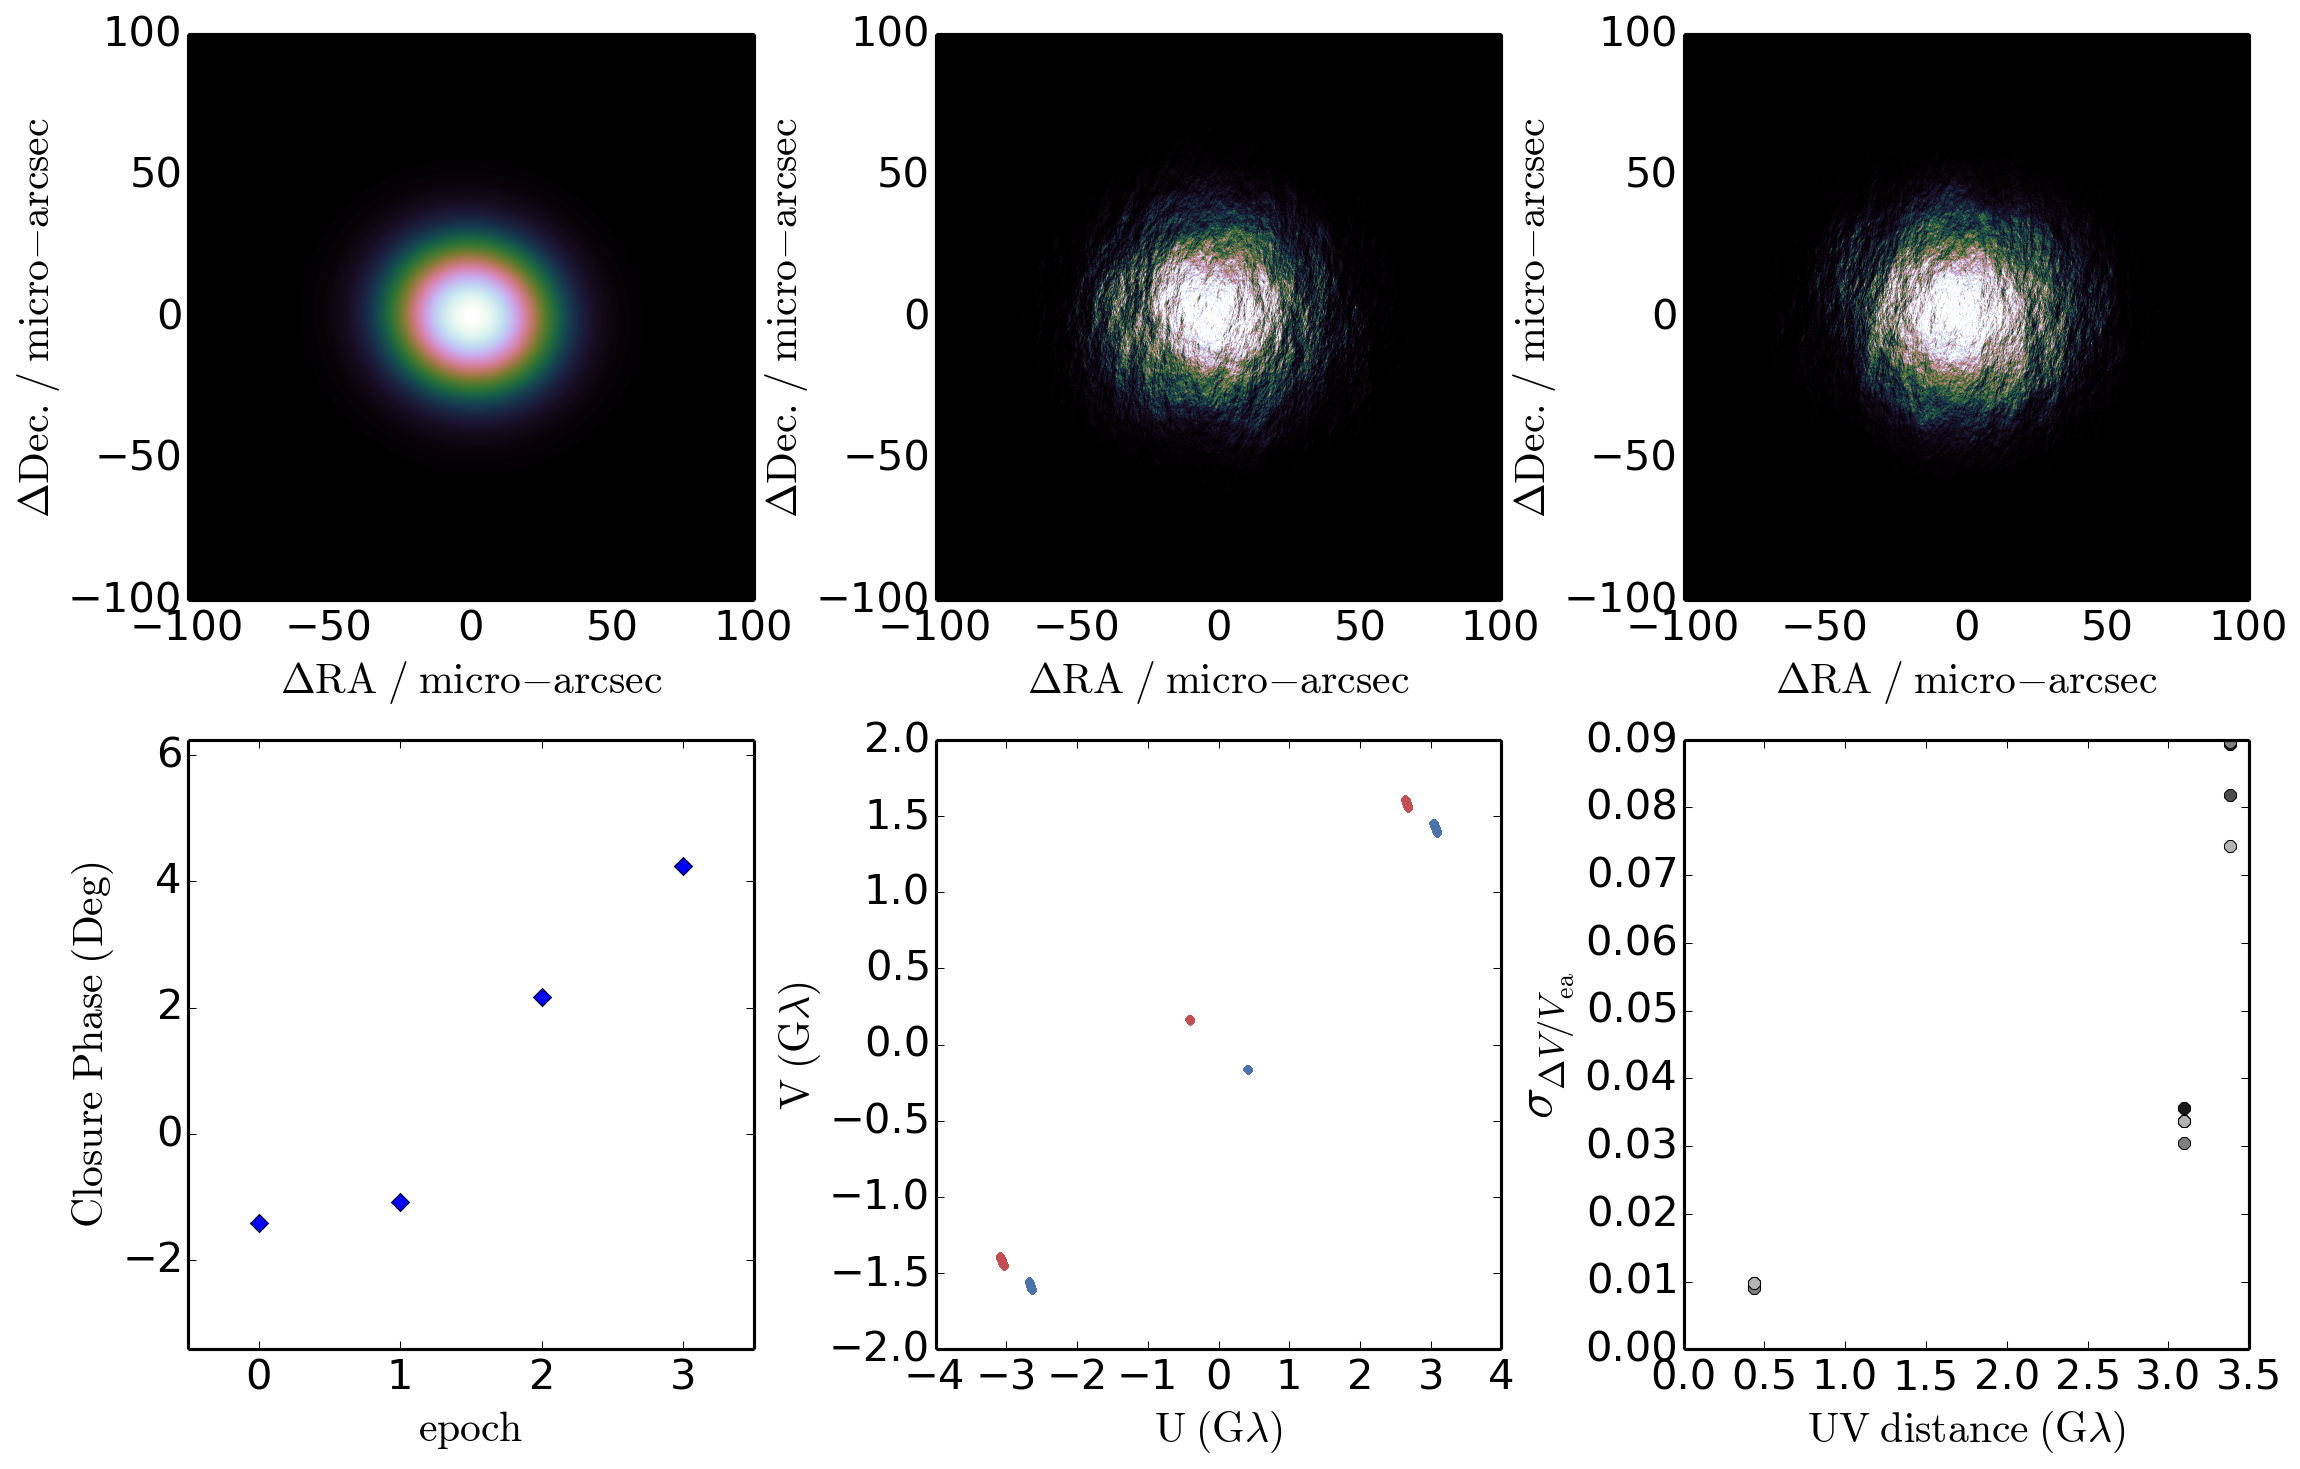
\includegraphics[width=1.8\columnwidth]{ism}
\caption{An example simulation of ISM scattering towards Sgr~A$^{\star}$, observed with SMT-JCMT-CARMA.  The top panel, left to right, shows the original $\rm FWHM = 40$~$\mu$-arcsec Gaussian {\bf (top left)}, the simulated ISM scattered image on the first night {\bf (top middle)} and last night {\bf (top right)} of the observation, respectively.  The bottom panel, left to right,  shows the evolution of the 10 minute-averaged closure phase with epoch {\bf (bottom left)}, {\sl uv}-tracks for each night {\bf (bottom middle)} and the RMS fractional visibility amplitude differences $\sigma_{\Delta V /V_{\rm ea}}$ as a function of {\sl uv-}distance {\bf (bottom right)}. $ \Delta V= (|V_{\rm a}|-|V_{\rm ea}|)$, where $|V_{\rm a}|$ and |$|V_{\rm ea}|$ are the simulated average and ensemble average visibility amplitudes respectively. Variations from the ensemble-average flux on the shortest baselines reveal total flux modulation while flux variations on longer baselines and non-zero closure phases track the fluctuations in substructure.  Furthermore, ISM scattering simulations can constrain the variability fraction associated with the screen, enabling a more robust estimation of source variability, as demonstrated in \citet{2016arXiv160106571O}. The time-variability of the ISM is built into the {\sc MeqSilhouette} framework.\label{ISM_sequence}%
}
\end{center}
\end{figure*}

\subsection{Atmospheric}

%Opacity + Brightness temperature
Typical opacities and sky brightness temperatures for ALMA, the Submillimeter Array (SMA) and the South Pole Telescope (SPT)  are shown in Fig.~\ref{fig:mean_atm}.  Note that both the opacity and brightness temperature are inversely proportional to the ground temperature and proportional to ground pressure.

\begin{figure}
\begin{center}
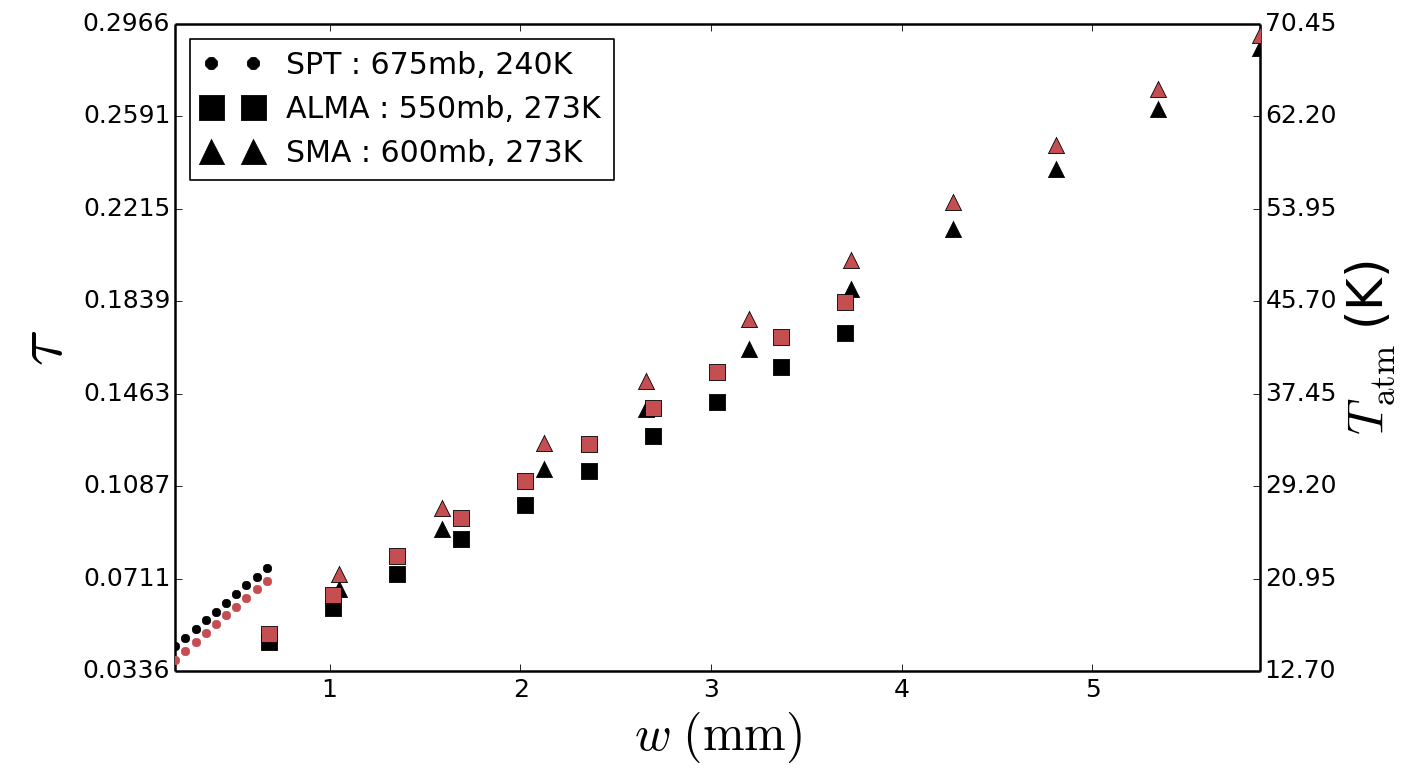
\includegraphics[width=1.\columnwidth]{Images/opacity}
\caption{Simulated mean opacity (black) and sky brightness temperature (red) at $\nu =230$~GHz  for three typical ground pressures and temperatures over a typical PWV range \citep{Lane_1998} which approximately represent the sites of SPT (dots), ALMA (squares) and SMA (triangles). The legend shows the estimated input ground (pressure, temperature) parameters for each site.\label{fig:mean_atm}%
}
\end{center}
\end{figure}


%Turbulent and mean delay
\begin{figure}
\begin{center}
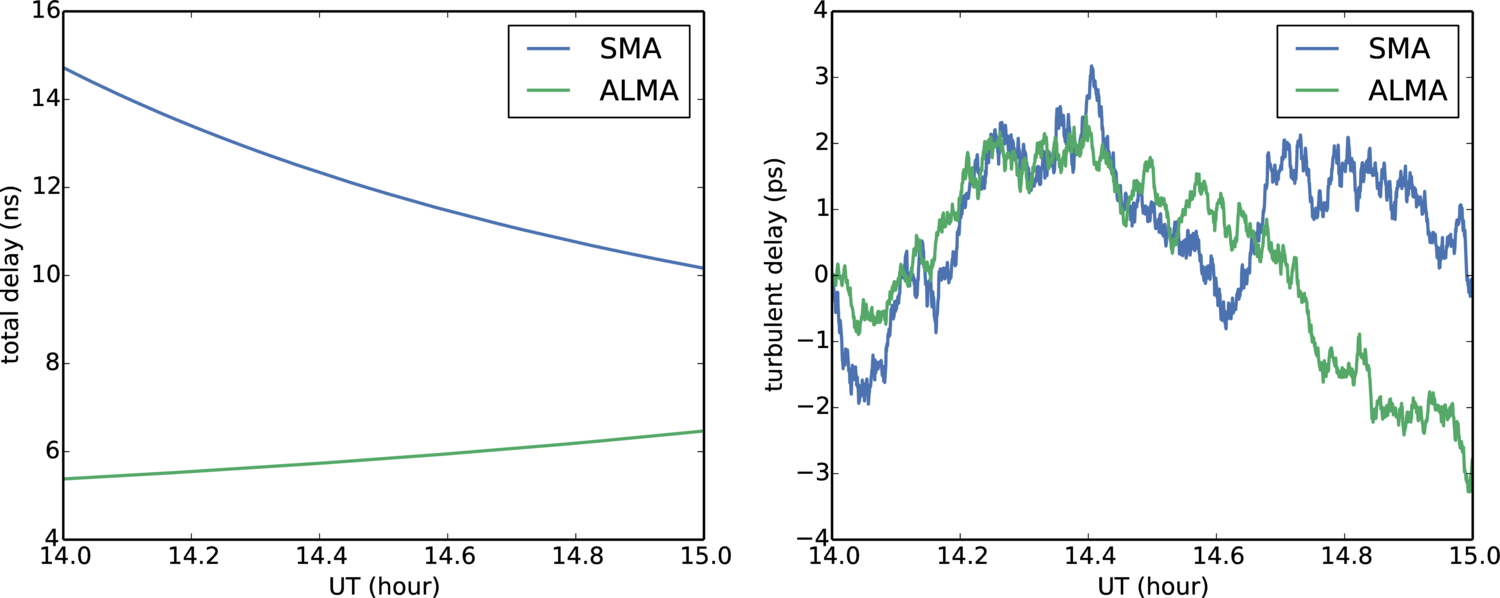
\includegraphics[width=\columnwidth]{Images/delays}
\caption{Simulation of the total delay (left) and the turbulent atmospheric delay (right) for SMA (blue) and ALMA (green) sites towards Sgr~A$^\star$. Ground pressures and temperatures are the same as Fig.~\ref{fig:mean_atm}, precipitable water vapour above each station is set to $w=2$~mm, and the instantaneous zenith coherence time is set $T_0=10$~s for both stations. Note that all tropospheric parameters are, however, independently set. The conversion from time delay to phase at 230~GHz is $1$~rad~$=0.7$~ps.\label{delay_plots}%
}
\end{center}
\end{figure}


%Trop images
\begin{figure*}
\begin{center}
\includegraphics[width=\columnwidth]{Images/trop_images}
\caption{The effect of residual troposphere phase noise on interferometric images of a point source observed for 12 hours at 230~GHz with 4~GHz bandwidth with the following array : SPT, ALMA, SMA, SMT, LMT and JCMT, assuming the same SEFDs as \protect\citet{Lu_2014} and an elevation limit of 15$^\circ$. For simplicity the weather parameters at each station were set to: coherence time $t_{\rm 0}=10$~sec; PWV depth $w=1$~mm; ground pressure $P=600$~mb; ground temperature $T =273$~K. {\bf Top left:} interferometric map with thermal noise only. {\bf Top right:} atmospheric attenuation and sky noise (due to non-zero opacity) with 1\% of the turbulent phase noise added. {\bf Bottom left:} as previous but with 3\% of turbulent phase contribution. {\bf Bottom right:} as previous but with 6\% turbulent phase contribution. The fractional turbulent phase contributions are illustrative of the effect of fringe-fitting errors. Note the decrease in the source peak flux with increasing turbulent tropospheric phase noise. Note further that the peak source centroid is offset from its true position (black crosshairs). \label{fig:trop_images}%
}
\end{center}
\end{figure*}


In section~\ref{sec:trop_errors} we explore the observational consequences of observing through a turbulent troposphere. In this simulation, we assume a simple point source model and apply increasing levels of turbulence-induced phase fluctuations before imaging using the two dimensional inverse fast Fourier transforms. We note a rapid attenuation in peak flux due to incoherent averaging, slight offsets in the source centroid and the presence of spurious imaging artefacts. Suprisingly, in this configuration, there was no evidence of blurring or a loss of resolution with the uncertainties. In an upcoming paper, we perform a systematic exploration of the turbulent tropospheric effects on the accuracy of fringe-fitting algorithms/strategies, through use of an automated calibration procedure and including the added complexity of a time-variable source. 


%Incoherent closure phases.. This section is needed to link up to the discussion on closure phase uncertainty in the mm-VLBI section

\subsection{Pointing}

\begin{figure}
\begin{center}
\includegraphics[width=\columnwidth]{Images/point_Crop}
\caption{RMS relative amplitude error induced by pointing error with the 50~m (i.e. fully illuminated) LMT antenna as a function of pointing error offset $\rho$ at 230~GHz. We assume that these errors are degenerate or non-separable from the self-calibration/fringe-fitting model used. See text for the description of the three models used. This simulation capability enables constraints on the magnitude of pointing-induced errors given a particular pointing calibration strategy.\label{fig:pointing}%
}
\end{center}
\end{figure}


In section~\ref{sec:pointing}, we show how antenna pointing errors of the LMT could introduce fractional RMS amplitude variations $\sigma_{\Delta V/V_0} \le 0.4$ on the timescale of phase centre switching. This would occur if the calibrator is widely separated from the source, as is often the case in mm-VLBI. In contrast tracking errors are less problematic with $\sigma_{\Delta V/V_0} \le 0.05$. If the gain error is non-separable from the calibration model used, it could be interpreted as intrinsic variability, substructure and/or increased noise. If unaccounted for, this effect has the potential to limit the dynamic range of mm-VLBI images. Further tests to constrain the pointing uncertainties of EHT stations will lead to more accurate interferometric simulations and hence the overall impact on black hole shadow parameter estimation. Here we demonstrate the capability to incorporate a range of plausible pointing error effects into a full simulation pipeline.  




 


\section{Calibration and imaging of a time variable source in the presence of the troposphere}

First we fringe fit and image a stationary point source and compare to the result in Fig.~\ref{fig:trop_images}. 








